\section{Viewer 3D}

\begin{frame}{Viewer 3D}
  Al fine di valutare \alert{qualitativamente} la validità dell'algoritmo di calibrazione delle ancore e di trilaterazione
  durante l'esecuzione di un esperimento è stato sviluppato un viewer 3D.\\
  Tale viewer consente di visualizzare la posizione cartesiana di uno o più tag
  mediante uno scatter plot.\\
  Inoltre il software è in grado di ricevere da uno dei tag la posizione delle ancore ottenuta
  mediante la procedura di calibrazione (procedura F. Fioretti) e di visualizzarne la posizione.\\
  Nel seguito è descritta brevemente l'architettura del software ed i metodi più importanti delle classi Python che ne
  costituiscono l'implementazione.
\end{frame}

\begin{frame}{Screenshot}
  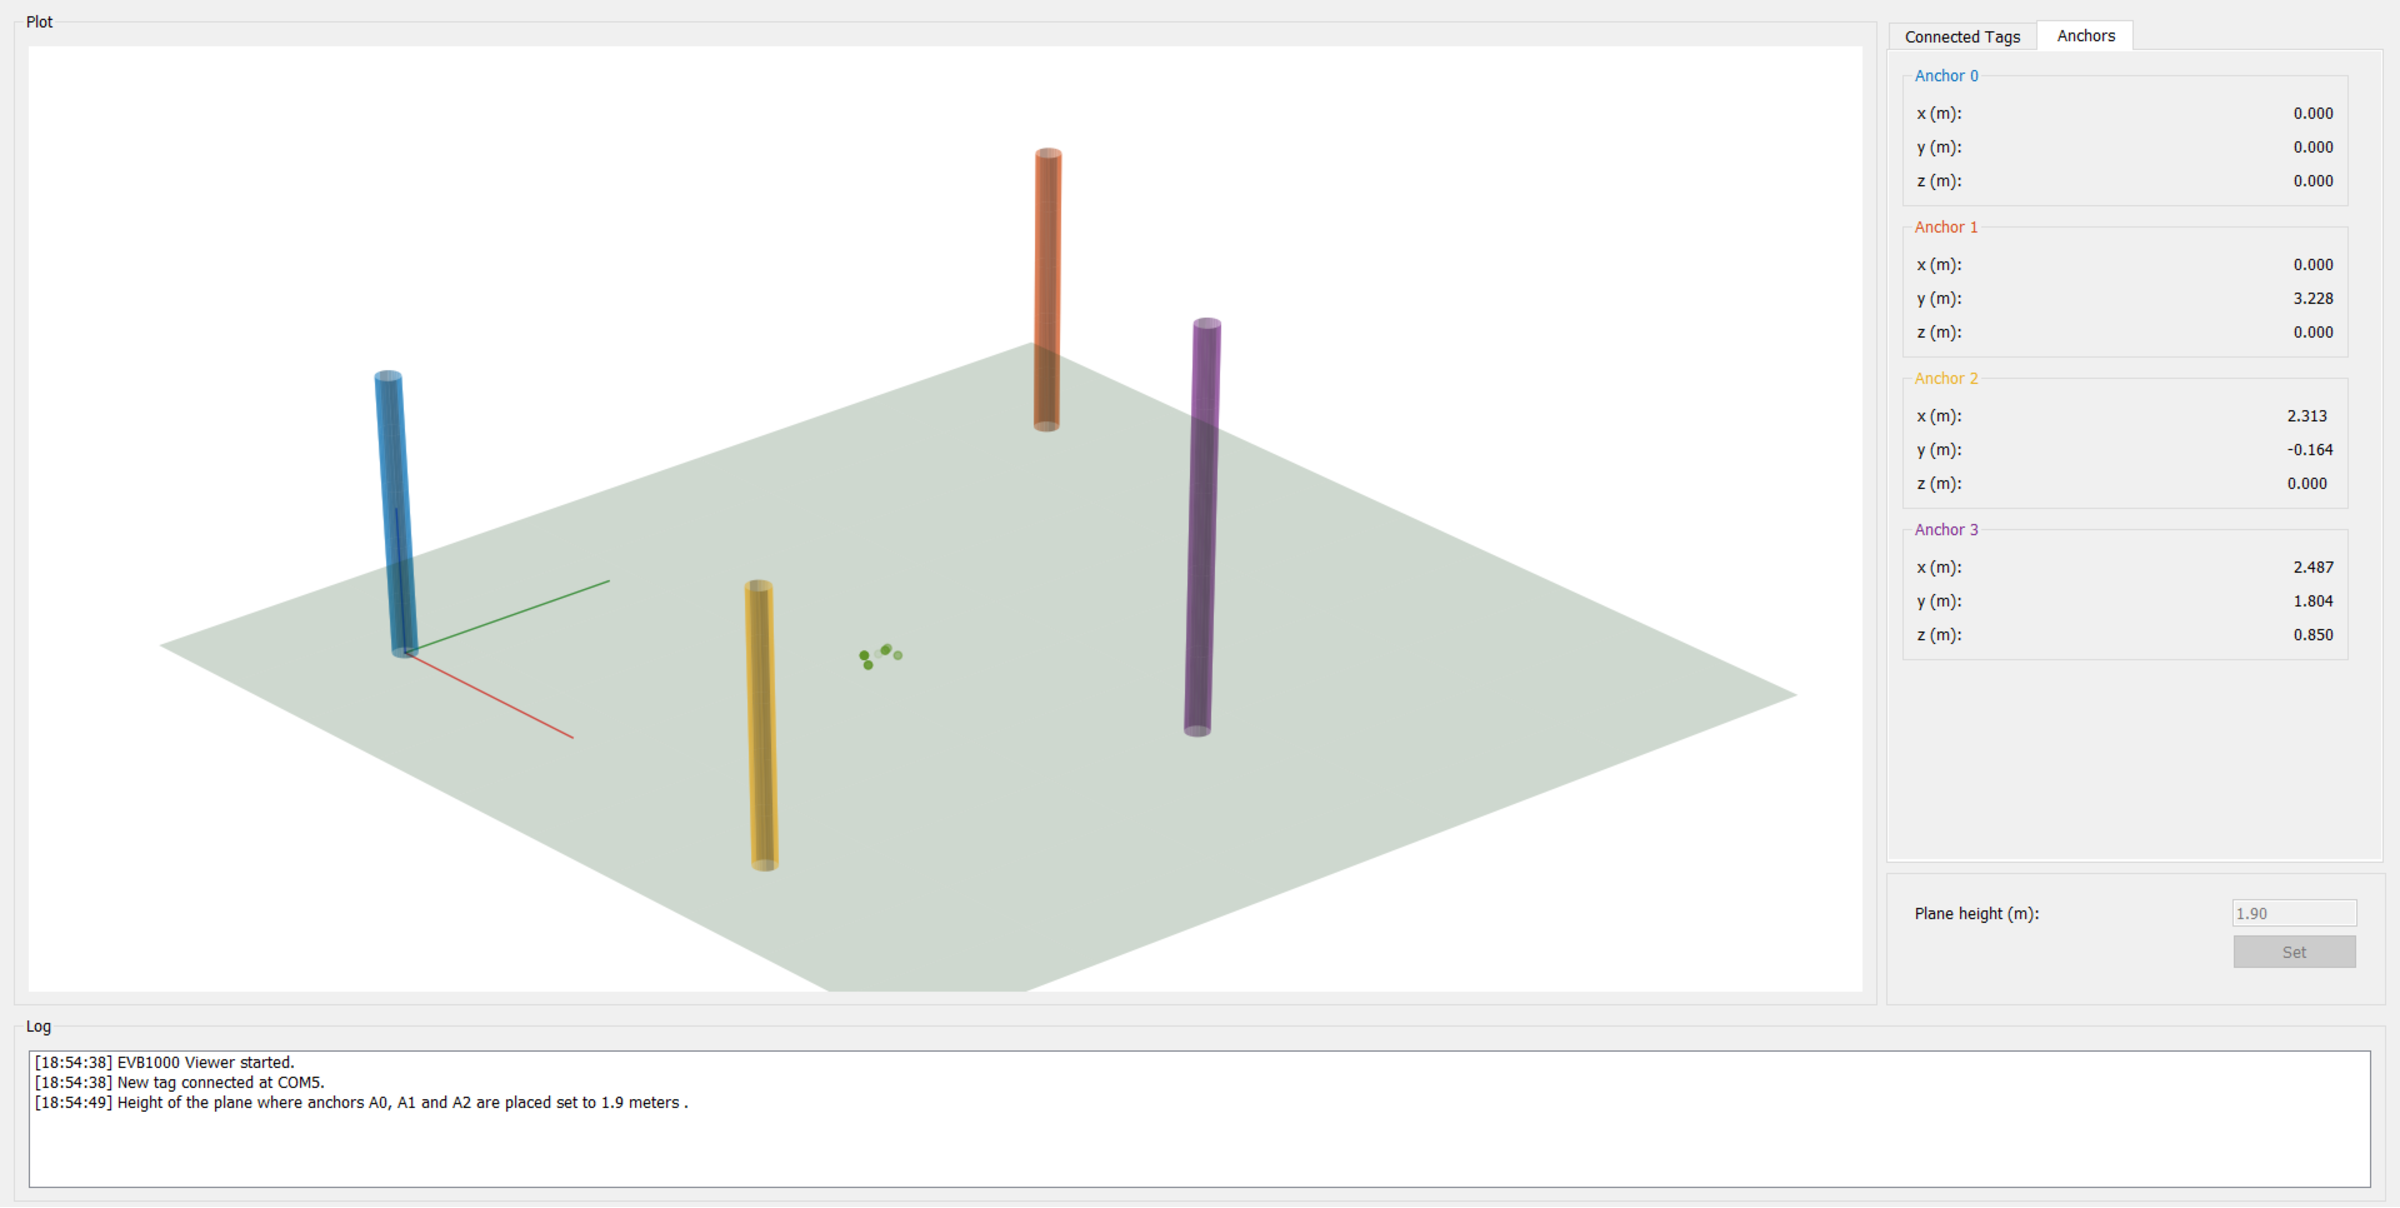
\includegraphics[width=\linewidth]{viewer_screenshot}
\end{frame}

\begin{frame}{Architettura}
  L'architettura prevede tre livelli:
  \begin{itemize}
  \item[-] gestione dei dispositivi (\textcolor{red}{Device Manager})
  \item[-] raccolta e decodifica dei dati (\textcolor{dgreen}{Device $i$-esimo})
  \item[-] visualizzazione dei dati (\textcolor{blue}{GUI, Canvas})
  \end{itemize}
  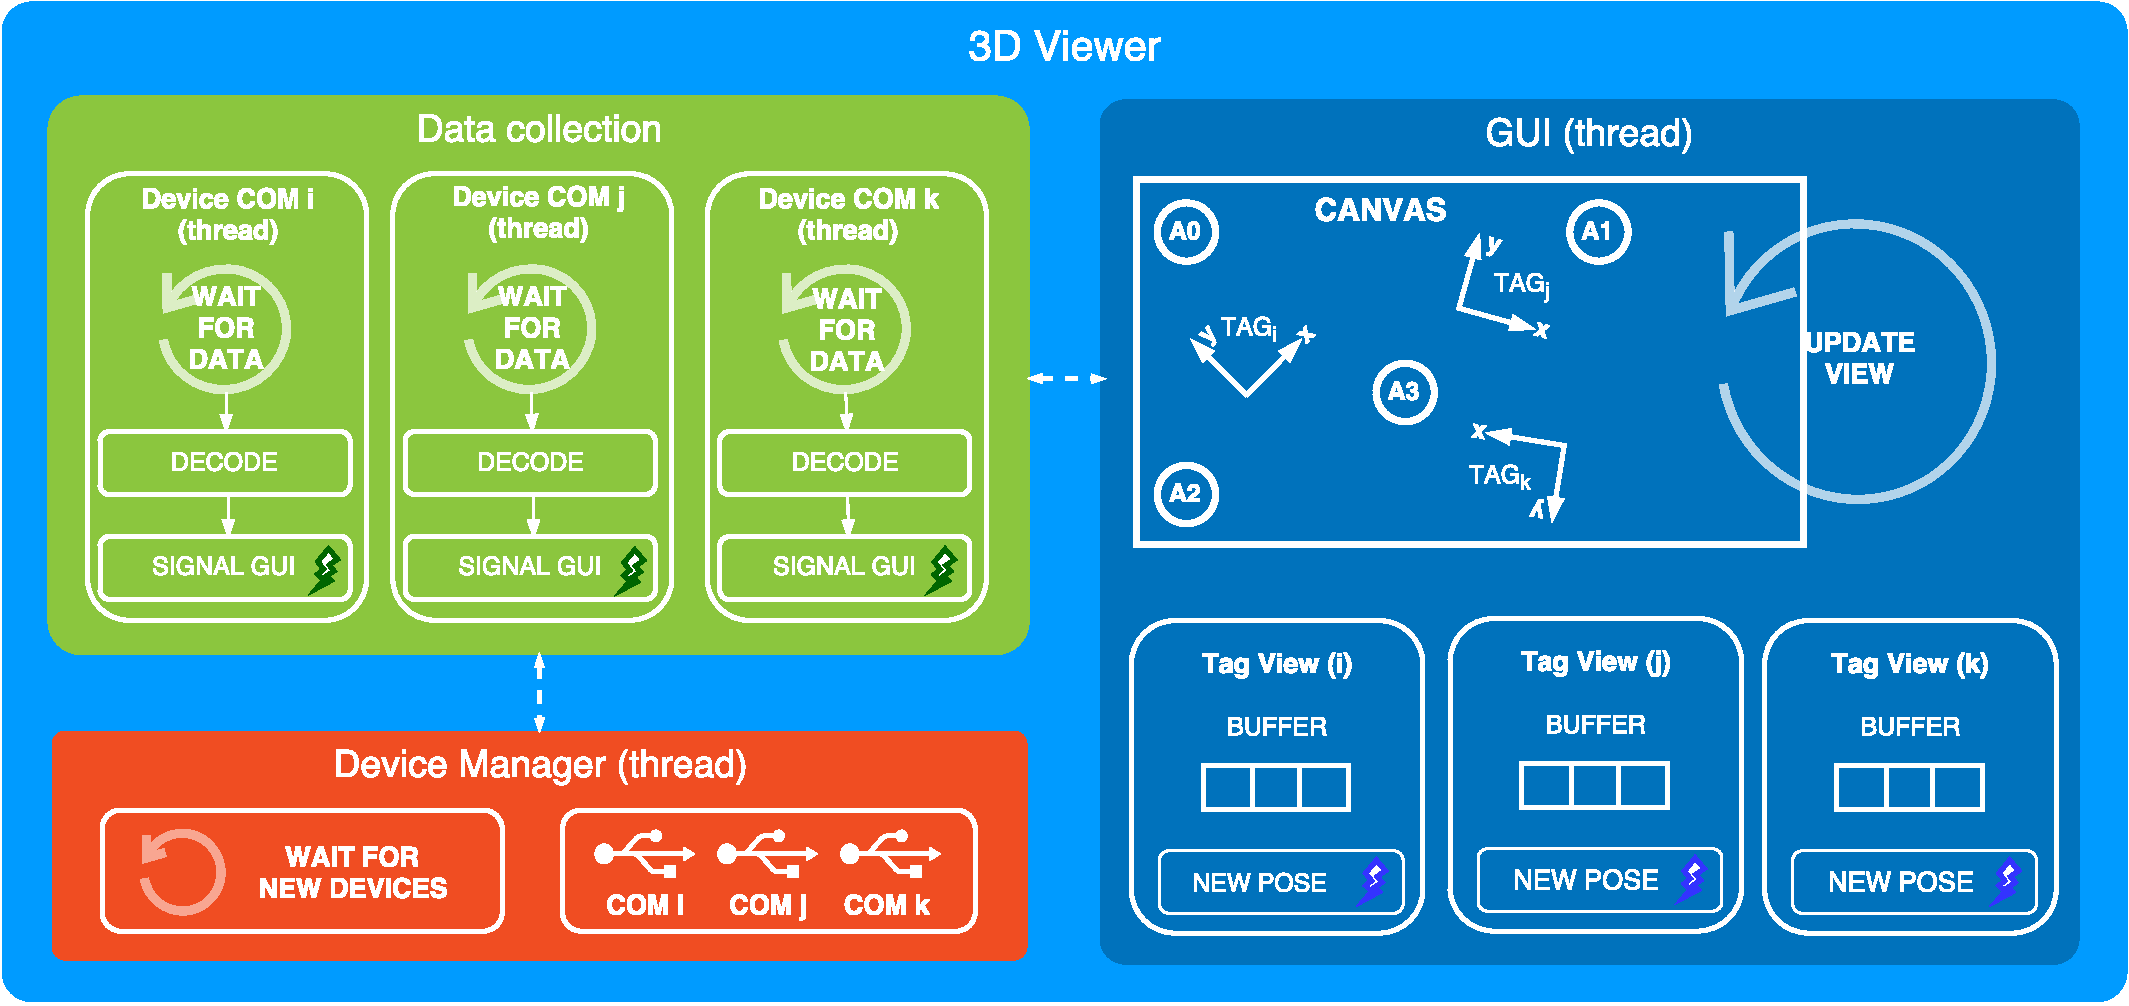
\includegraphics[width=\linewidth]{viewer_arch}
\end{frame}

\begin{frame}[shrink=10]{Architettura - Device Manager}
  \begin{center}
    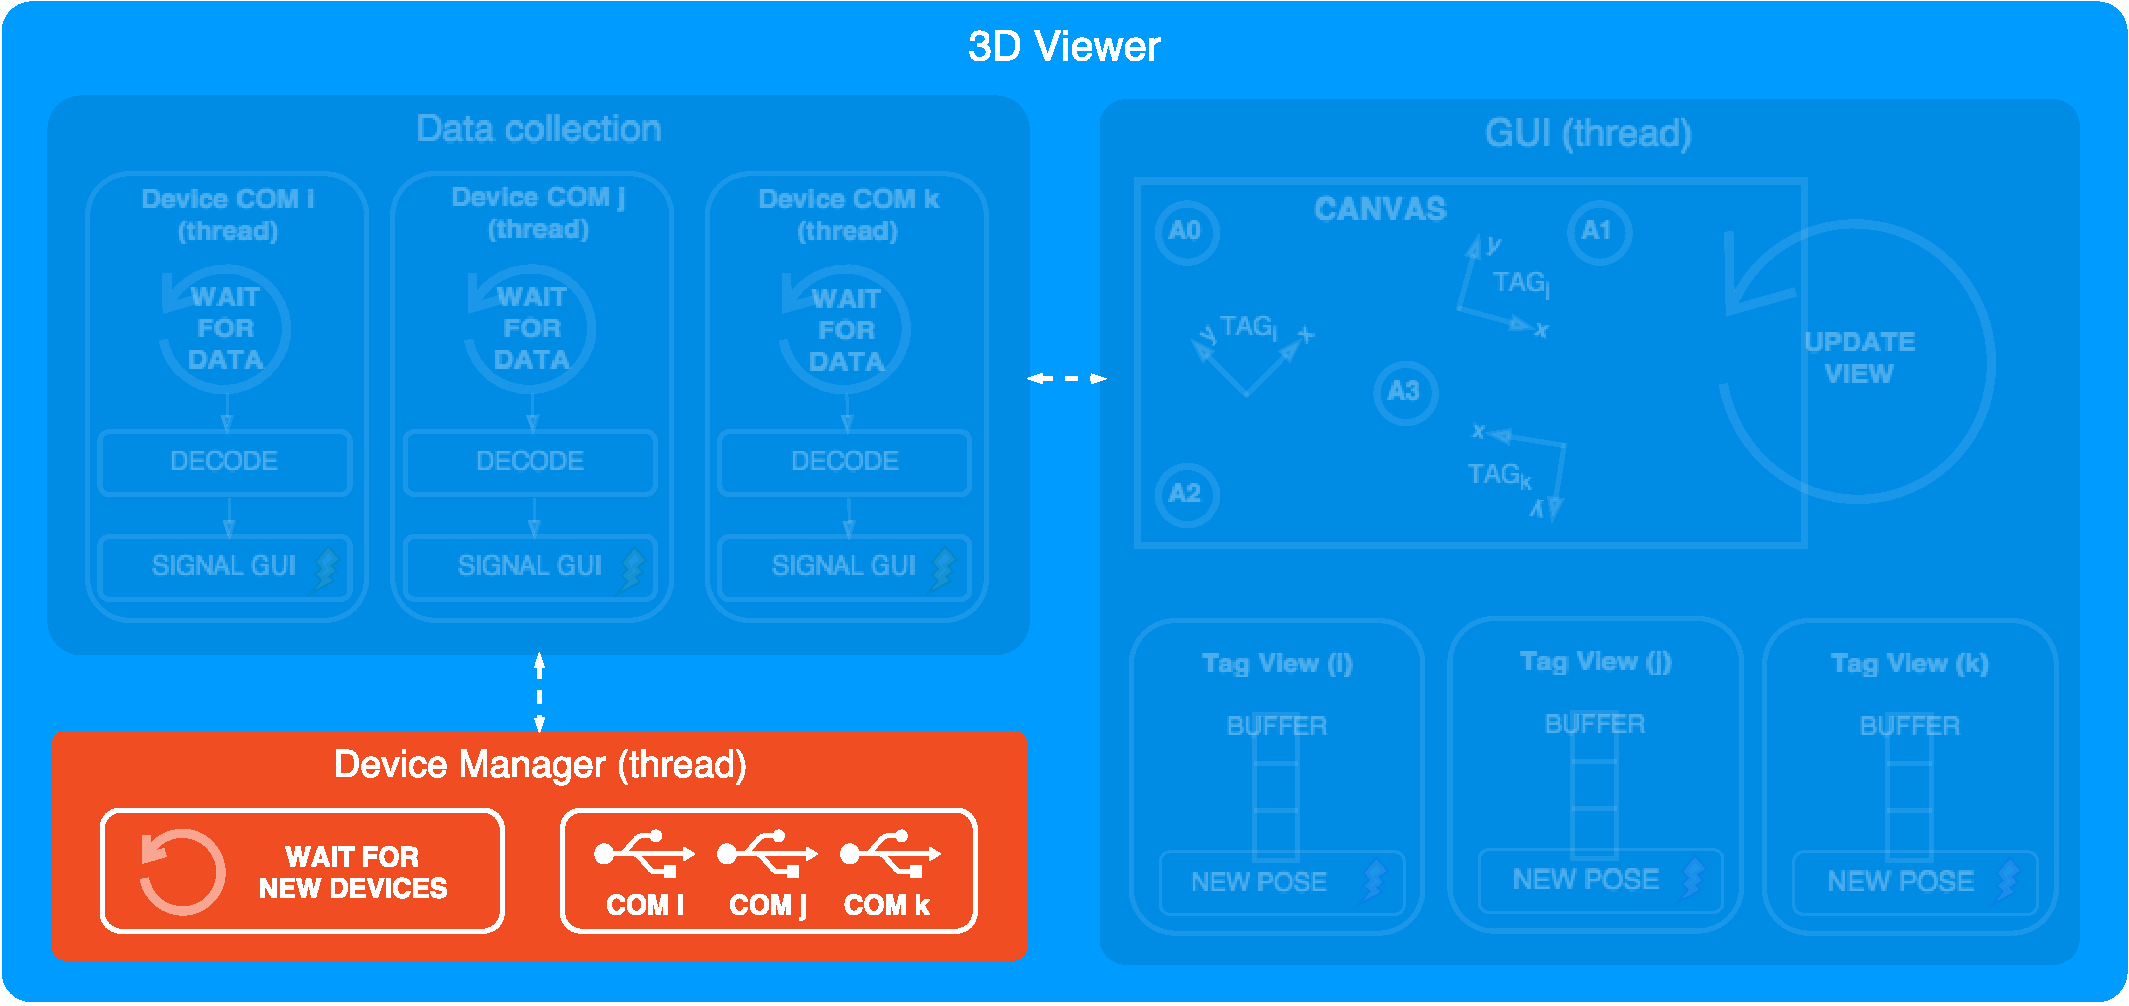
\includegraphics[height=10em]{viewer_arch_dev_man_only}
  \end{center}
  Il Device Manager si occupa di rilevare periodicamente nuovi dispositivi connessi al computer tramite porta seriale
  (reale o virtuale).\\
  Per ogni nuovo dispositivo connesso vengono allocate apposite strutture dati e creato un thread che si occupa della gestione
  dei dati in arrivo.\\
  Quando un dispositivo viene disconnesso il thread ad esso associato viene terminato.
\end{frame}

\begin{frame}[fragile, shrink=30, label={device_thread_loop}]{Implementazione - classe \lstinline!DeviceManager! - metodo \lstinline!run()!}
  \begin{center}
    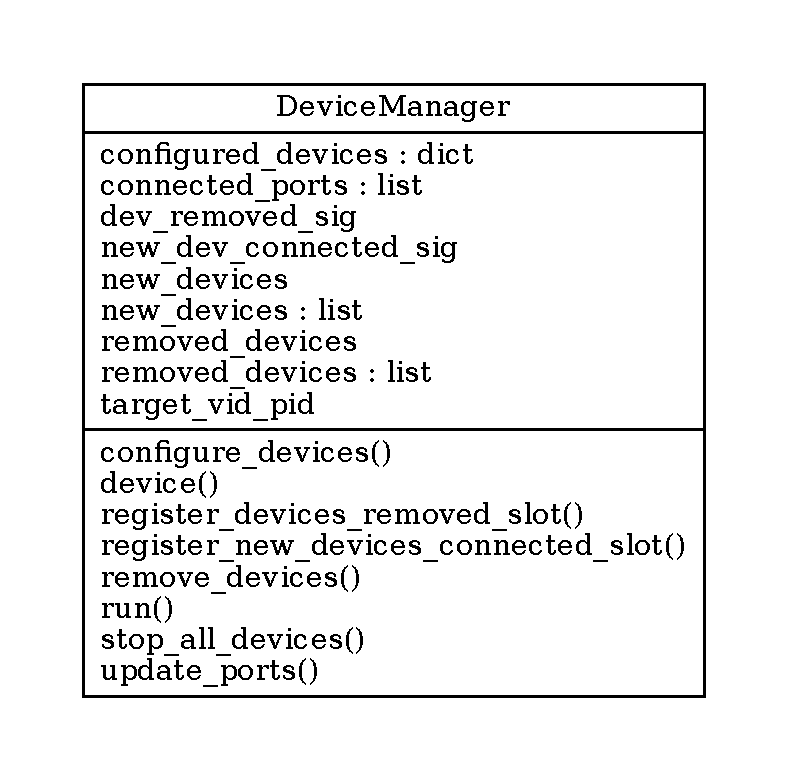
\includegraphics[height=12em]{device_manager}
  \end{center}
  \vskip -3em
  Il metodo \lstinline!run! è il metodo principale associato al thread del Device Manager.\\
  \begin{Python}
    def run(self):
        while True:
            new_ports, removed_ports = self.update_ports()
  \end{Python}
  Il metodo \lstinline!update_ports()! rileva le nuove porte seriali connesse e le porte che sono
  state scollegate di recente.\\
  Per ogni nuova porta la funzione \lstinline!configure_devices()! si occupa di \alert{generare
  un'istanza della classe \lstinline!Device!.}
  \begin{Python}
            if new_ports:
                self.new_devices = self.configure_devices(new_ports)
  \end{Python}
\end{frame}

\begin{frame}[fragile, shrink=10]{Implementazione - classe \lstinline!DeviceManager! - metodo \lstinline!run()!}
  Inoltre viene emesso un \alert{segnale} per notificare l'evento alla GUI. Nel seguito verrà
  spiegato in che modo la GUI si registra agli eventi emessi dal Device Manager.

  \begin{Python}
                self.new_dev_connected_sig.emit()
  \end{Python}
  Per ogni porta scollegata la funzione \lstinline!remove_devices()! si occupa di 
  terminare il thread associato a tale porta. Inoltre la GUI viene notificata dell'evento.
  \begin{Python}
            if removed_ports:
                self.removed_devices = self.remove_devices(removed_ports)
                self.dev_removed_sig.emit()
  \end{Python}
  Il thread del Device Manager esegue periodicamente con frequenza di \SI{1}{\hertz}.
  \begin{Python}
            sleep(1)
  \end{Python}
  
\end{frame}

\begin{frame}[shrink=10]{Implementazione - classe \lstinline!DeviceVIDPIDList!}
  \begin{center}
    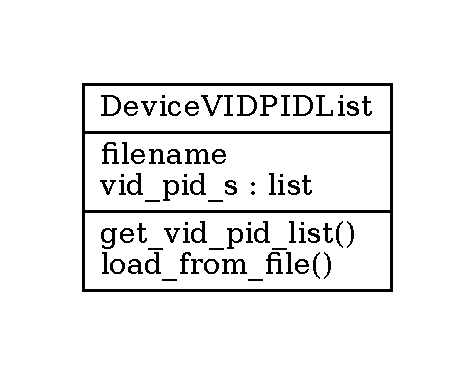
\includegraphics[height=10em]{vidpidlist}
  \end{center}
  Per poter rilevare i nuovi dispositivi connessi \alert{di interesse} il Device Manager necessita
  di conoscere il \lstinline!VID (Vendor ID)! e \lstinline!PID (Product ID)! associati alla porta
  USB della porta seriale utilizzata. Una classe \lstinline!DeviceVIDPIDList! si occupa di caricare
  un elenco di ID desiderati da un file di configurazione.\\
  Un'istanza della classe \lstinline!DeviceVIDPIDList! viene passata all'istanza della classe
  \lstinline!DeviceManager! al momento della sua costruzione.
\end{frame}

\begin{frame}[fragile]{Implementazione - file di configurazione}
  La struttura del file di configurazione è molto semplice ed è la seguente
  \begin{lstlisting}
    CONFIG_VID_PID
    VID PID
    <vid 1> <pid 1>
    ...
    <vid N> <pid N>
  \end{lstlisting}
  dove \lstinline!<vid i>! e \lstinline!<pid i>! sono dati ciascuno da
  una sequenza di $4$ cifre. Ad esempio
  \begin{lstlisting}
    CONFIG_VID_PID
    VID PID
    0483 5740
  \end{lstlisting}

\end{frame}

\begin{frame}[fragile, shrink=10]{Architettura - Device $i$-esimo}
  \begin{center}
    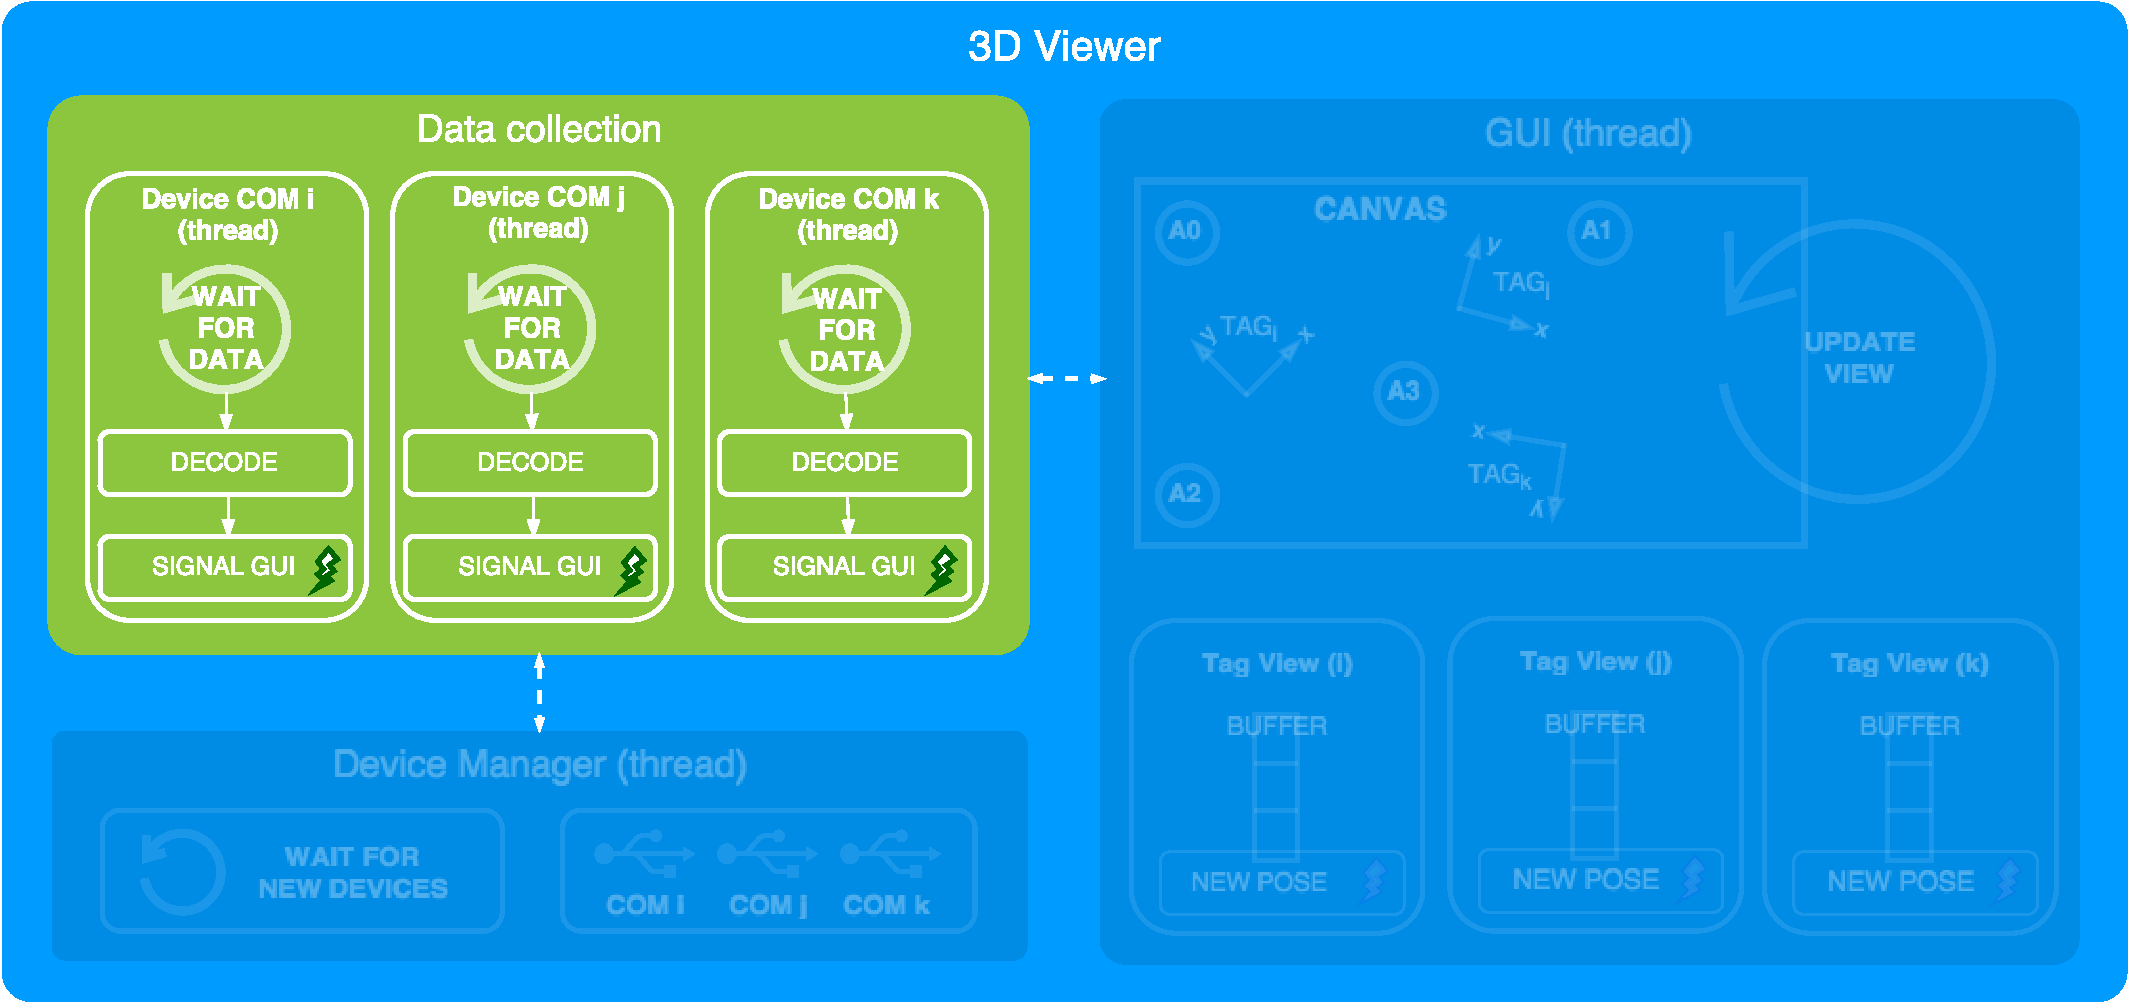
\includegraphics[height=10em]{viewer_arch_device_only}
  \end{center}
  Un thread viene associato ad ogni dispositivo connesso. Esso si occupa di interrogare continuamente
  la porta seriale associata al dispositivo e di decodificare ogni nuova linea, terminata da \lstinline!\r\n!,
  ricevuta.\\
  Se la decodifica avviene con successo il thread, mediante un meccanismo di signal-slot, notifica alla GUI
  la presenza di nuovi dati.
\end{frame}

\begin{frame}[fragile, shrink=30]{Implementazione - classe \lstinline!Device! - \lstinline!run()!}
  \begin{center}
    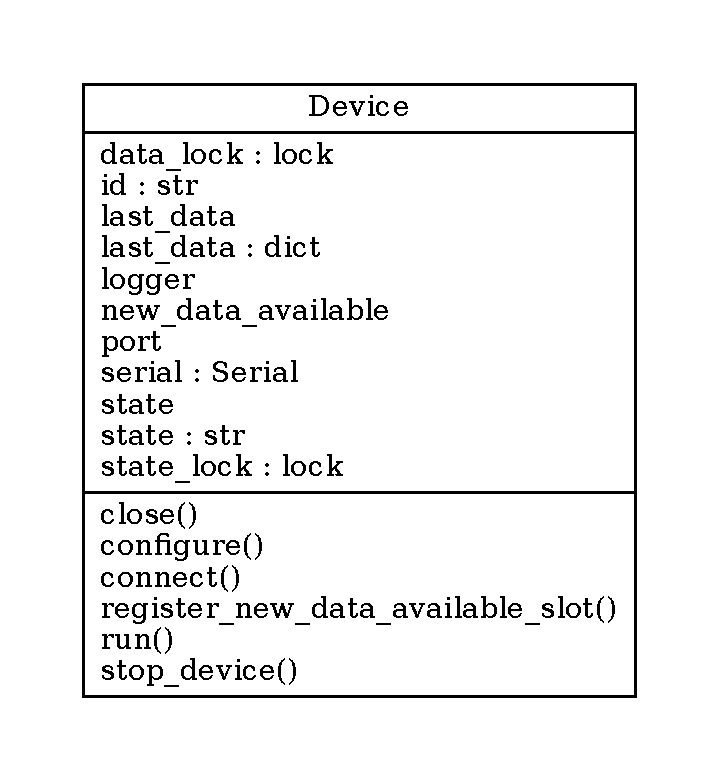
\includegraphics[height=12em]{device}
  \end{center}
  \vskip -3em
  Il metodo \lstinline!run! è il metodo principale associato al thread di ciascun Device.\\
  Dopo aver verificato l'avvenuta connessione con la porta seriale
  \begin{Python}
    def run(self):
        if not self.connect():
            return
  \end{Python}
  il metodo entra nel loop principale dal quale esce solo nel caso in cui lo stato
  diventi \lstinline[language=Python]!stopped! (i.e. quando il Device Manager termina
  il thread)
  \begin{Python}
        while self.state == 'running':
  \end{Python}
\end{frame}
  
\begin{frame}[fragile, shrink=20]{Implementazione - classe \lstinline!Device! - \lstinline!run()!}
  Il metodo tenta quindi di leggere una linea terminata da \lstinline!\r\n!
  e di decodificarla attraverso la classe \lstinline!DataFromEVB1000!
  \begin{Python}
           try:
                line = self.serial.readline()
                if len(line) > 0:
                    try:
                        evb1000_data = DataFromEVB1000(line)
                    except InvalidDataFromEVB1000:
                        continue
  \end{Python}
  Nel caso di decodifica avvenuta con successo i nuovi dati sono memorizzati
  nel campo \lstinline!last_data! dell'istanza del \lstinline!Device!, la GUI
  viene notificata della presenza di nuovi dati
    \begin{Python}
                    if evb1000_data.msg_type_decoded:
                        self.last_data = evb1000_data.decoded
                        self.new_data_available.emit(self.id)
                        self.logger.log_data(evb1000_data)
    \end{Python}
\end{frame}

\begin{frame}[fragile, shrink=20]{Implementazione - classe \lstinline!Device! - \lstinline!run()!}\
  Nel caso di errore nella lettura da seriale i nuovi dati vengono scartati
  \begin{Python}
            except SerialException:
                pass
  \end{Python}

  Qualora lo stato del \lstinline!Device! diventi \lstinline!stopped!
  la porta seriale viene chiusa
  \begin{Python}
        if self.state == 'stopped':
            self.close()

  \end{Python}
\end{frame}

\begin{frame}[fragile, shrink=30]{Implementazione - classe \lstinline!DataFromEVB1000! - \lstinline!decode_msg_type()!}
  \begin{center}
    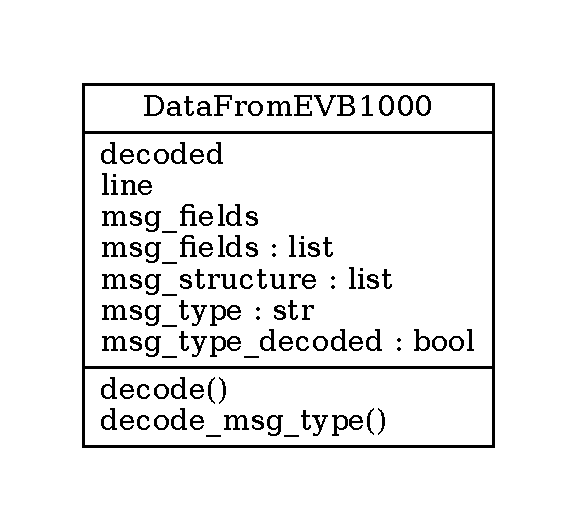
\includegraphics[height=12em]{data_from_evb1000}
  \end{center}
  \vskip -3em
  Il metodo fondamentale della classe \lstinline!DataFromEVB1000! è \lstinline!decode_msg_type!
  che definisce la struttura interna del messaggio ricevuto.\\
  Il tipo del messaggio è ricavato dai primi tre caratteri della linea \lstinline!line!
  \begin{Python}
      def decode_msg_type(self):
        if len(self.line) < 3:
            return False
        msg_type = self.line[0:3]
  \end{Python}
\end{frame}

\begin{frame}[fragile, shrink=30]{Implementazione - classe \lstinline!DataFromEVB1000! - \lstinline!decode_msg_type()!}
  Nel caso di un messaggio di tipo Tag Position Report il tipo è \lstinline!tpr!,
  
  \begin{Python}
        if msg_type == 'tpr':
  \end{Python}
  
  i campi del messaggio sono nominati \lstinline!msg_type!, \lstinline!tag_id! (i.e. l'id
  del tag come da switch sul PCB), \lstinline!x!, \lstinline!y! e \lstinline!z!
  \begin{Python}
            self.msg_fields = ['msg_type', 'tag_id', 'x', 'y', 'z']
  \end{Python}
  e i loro tipi sono indicati come \lstinline!s! (stringa), \lstinline!u! (unsigned int)
  e tre \lstinline!f! (float)
  \begin{Python}
            self.msg_structure = ['s'] + ['u'] + ['f'] * 3
  \end{Python}
  Altri tipi di messaggio sono indicati negli altri rami
  \begin{Python}
        elseif ...
  \end{Python}
  la decodifica fallisce qualora il tipo di messaggio non sia tra quelli riconosciuti
  \begin{Python}
        else:
            return False

        return True
  \end{Python}
\end{frame}

\begin{frame}[shrink=10]{Architettura - GUI}
  \begin{center}
    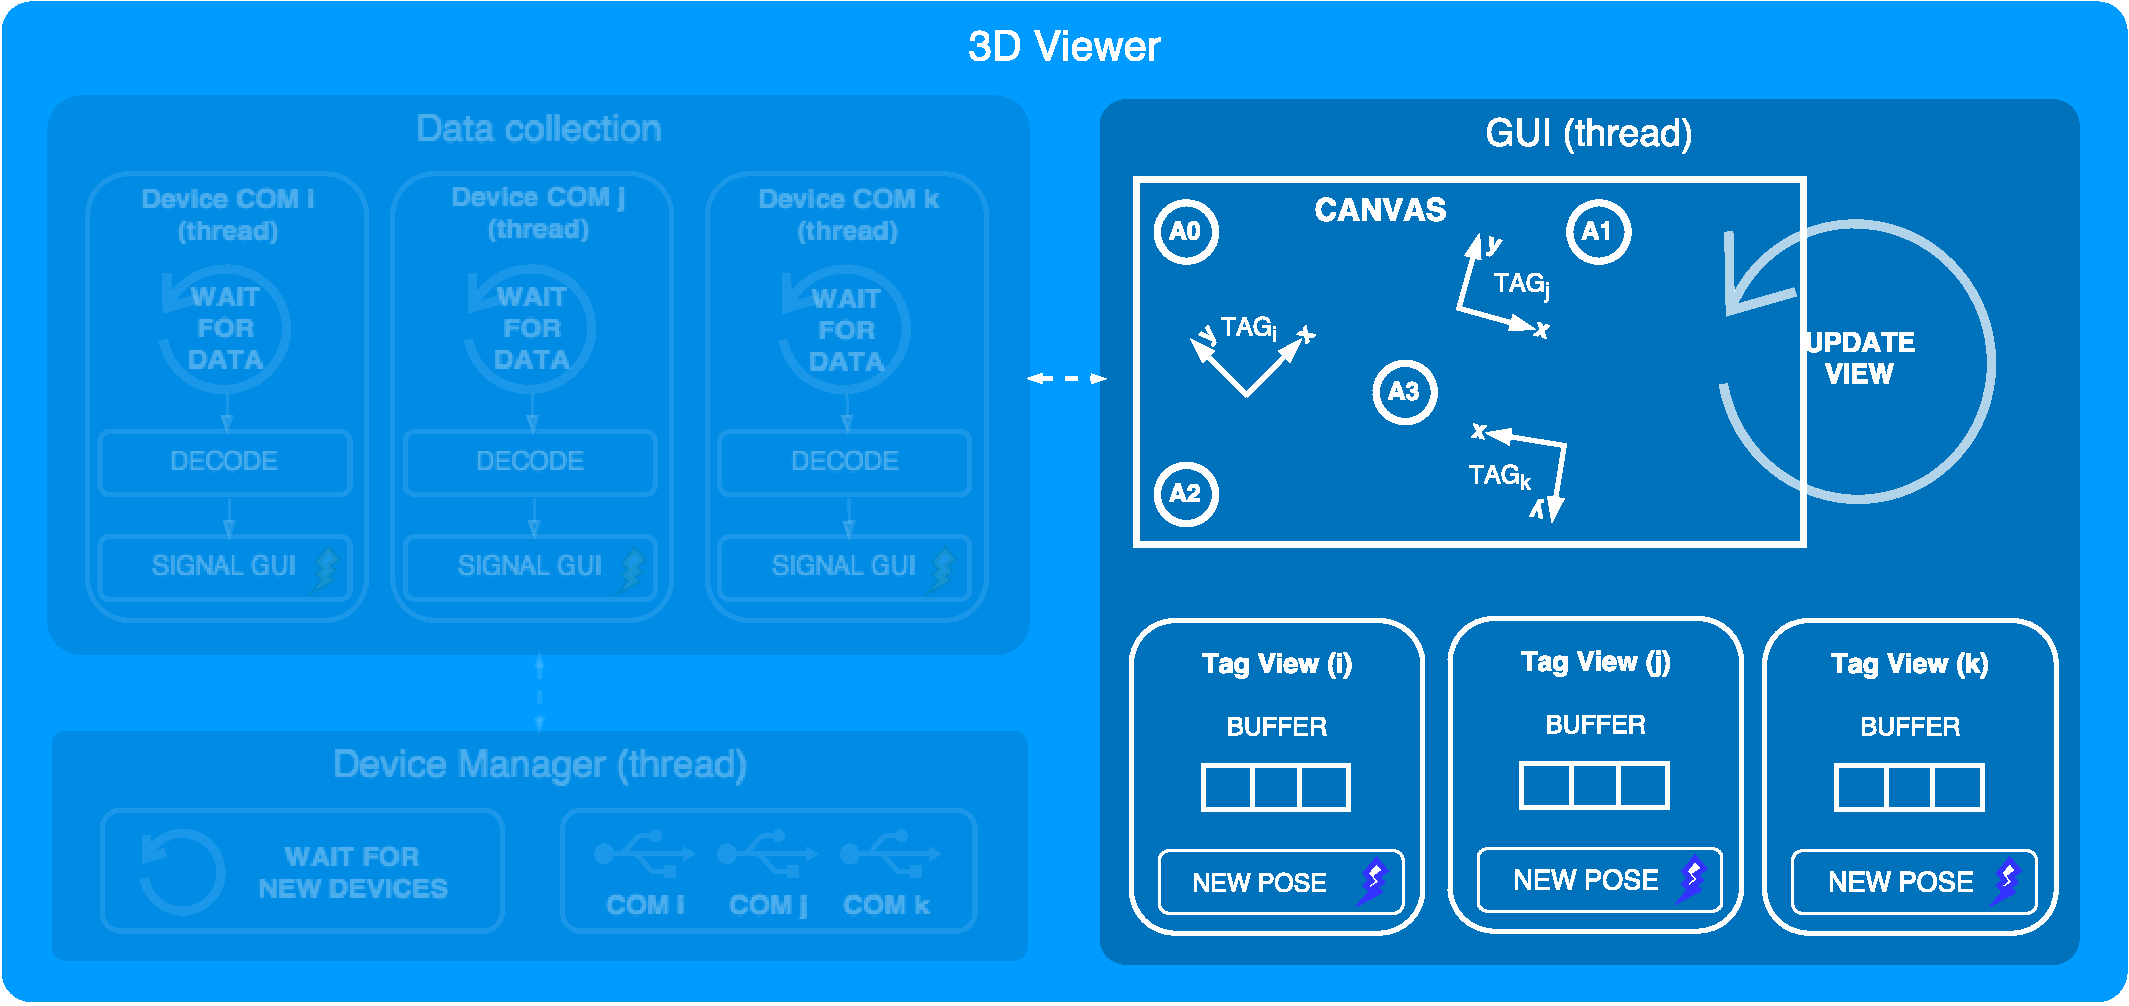
\includegraphics[height=10em]{viewer_arch_gui_only}
  \end{center}
  Per la GUI è previsto un thread a parte che, mediante callback dette slot, riceve le notifiche
  provenienti da ciascun Device thread e dal Device Manager.\\
  Quando una nuova posizione del tag è disponibile viene memorizzata all'interno di una struttura dati
  con buffer, detta Tag View. Una variante di Tag View, detta Tag Position Attitude View, è prevista
  per ospitare la stima di posizione e assetto.\\
\end{frame}

\begin{frame}[shrink=10]{Architettura - GUI}
  \begin{center}
    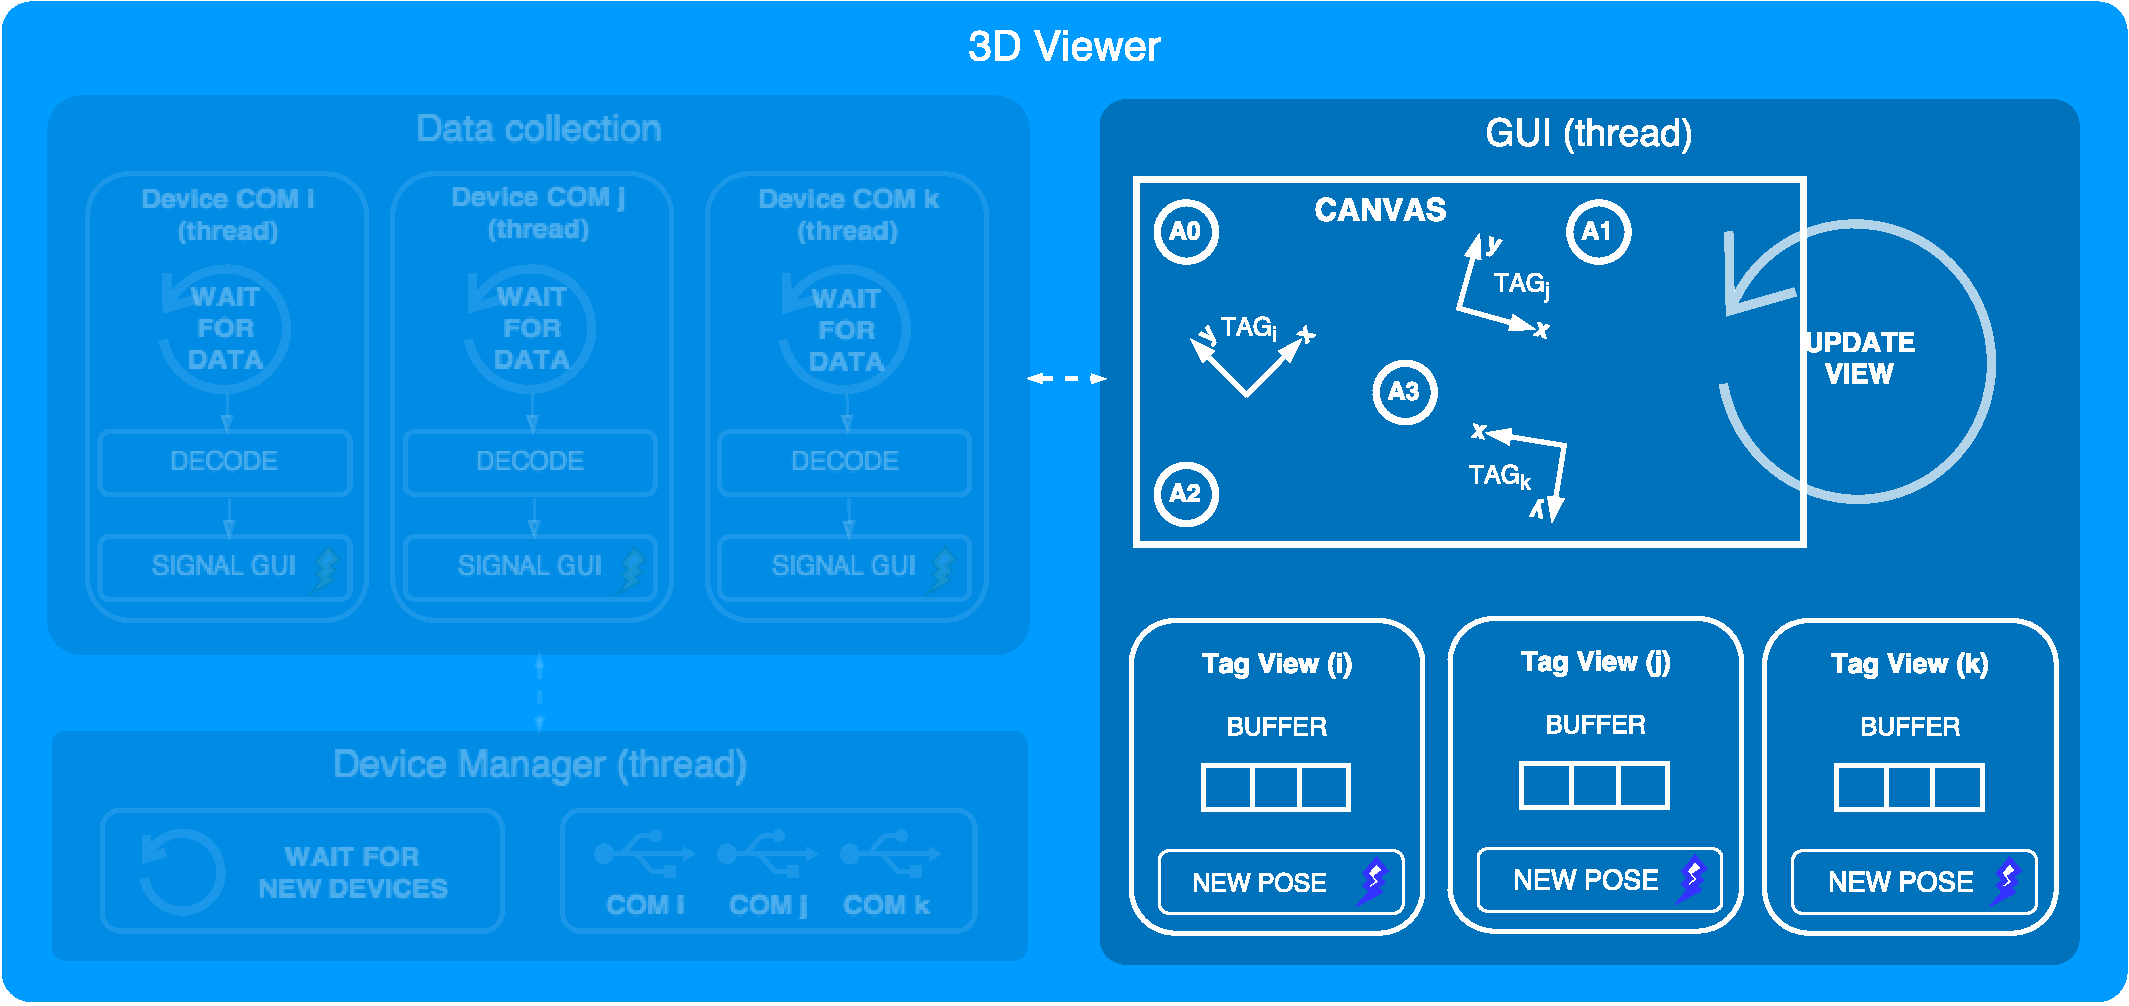
\includegraphics[height=10em]{viewer_arch_gui_only}
  \end{center}
  Periodicamente la GUI aggiorna il Canvas principale, ospitato nella finestra, in cui vengono rappresentate la posizione del tag con uno scatter 3D e la stima con una terna.\\
  Il Canvas prevede inoltre la rappresentazione delle ancore mediante dei cilindri. La posizione delle ancore
  viene trasmessa dal tag attraverso la porta seriale.
\end{frame}

\begin{frame}[shrink=15]{Implementazione - classe \lstinline!EVB1000ViewerMainWindow!}
  \begin{center}
    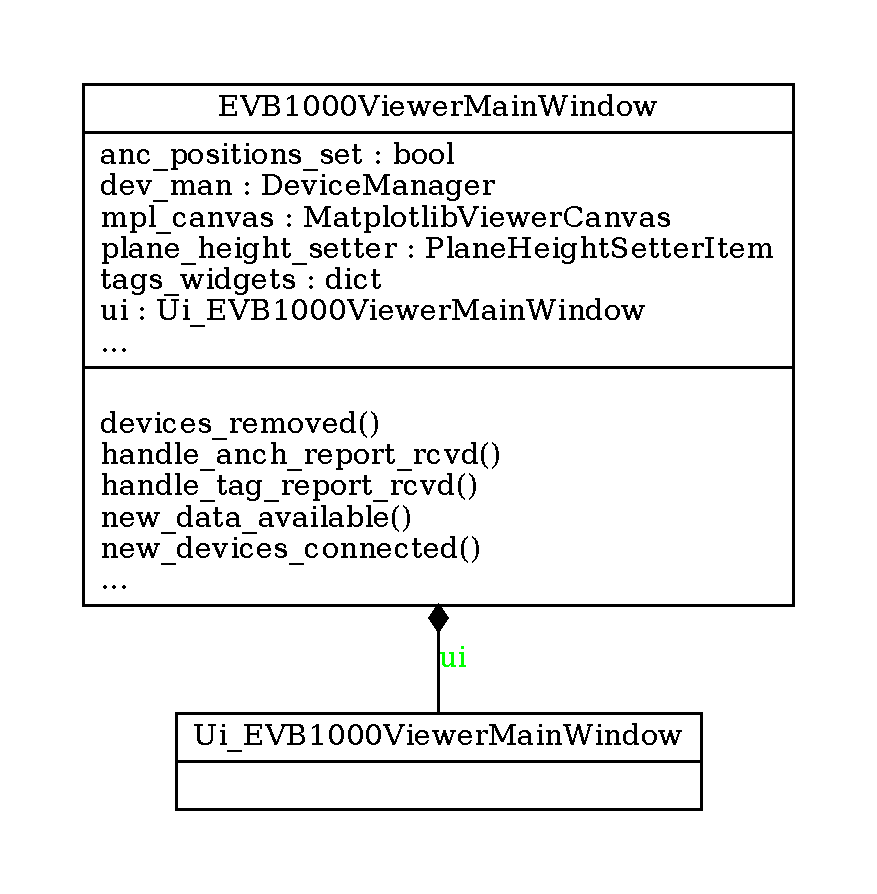
\includegraphics[height=12em]{evb1000_main_window}
  \end{center}
  \vskip -3em
  La classe fondamentale che implementa la GUI è \lstinline!EVB1000ViewerMainWindow!.\\
  Essa contiene un riferimento alla classe \lstinline!Ui_EVB1000ViewerMainWindow! che contiene
  l'implementazione della finestra principale generata dal software Qt Creator.\\
  Al fine di capire in che modo il Device Manager e il Device notificano alla GUI rispettivamente
  la presenza di nuovi dispositivi connessi e la presenza di nuovi dati è opportuno analizzare
  il costruttore della classe \lstinline!EVB1000ViewerMainWindow! ed i metodi \lstinline!new_devices_connected()!
  e \lstinline!new_data_available()!.
\end{frame}

\begin{frame}[fragile, shrink=15]{Implementazione - classe \lstinline!EVB1000ViewerMainWindow! -- \lstinline!costruttore!}
  Al costruttore della classe \lstinline!EVB1000ViewerMainWindow! viene passata
  un'istanza \lstinline!device_manager! del Device Manager
  \begin{Python}
    def __init__(self, device_manager = None):
        ...
  \end{Python}
  
  viene inizializzata/configurata la classe della finestra principale
  \begin{Python}
        self.ui = Ui_EVB1000ViewerMainWindow()
        self.ui.setupUi(self)
        ...
  \end{Python}

  viene creata un'istanza del Canvas che ospiterà la rappresentazione delle
  ancore e dei tag
  \begin{Python}
        frame_rate = 25.0
        tag_positions_buffer_size = 10
        self.mpl_canvas = MatplotlibViewerCanvas(self.ui.matPlotGroupBox,\
                                                 frame_rate,\
                                                 tag_positions_buffer_size)
        ...
  \end{Python}
\end{frame}

\begin{frame}[fragile, shrink=15]{Implementazione - classe \lstinline!EVB1000ViewerMainWindow! -- \lstinline!costruttore!}
  e viene salvato il riferimento al Device Manager 
  \begin{Python}
        self.dev_man = device_manager
  \end{Python}

  Molto \alert{importante} è la seguente parte in cui la GUI registra
  due metodi della classe come \lstinline!slot! associati a segnali emessi
  dal Device Manager.\\
  In pratica il metodo \lstinline!new_devices_connected! verrà richiamato quando il Device Manager
  rileva nuovi dispositivi connessi ed il metodo \lstinline!devices_removed! sarà richiamato
  quando alcuni dispositivi sono stati scollegati.
  \begin{Python}
        if self.dev_man != None:
            self.dev_man.register_new_devices_connected_slot(\
                         self.new_devices_connected)
            self.dev_man.register_devices_removed_slot(\
                         self.devices_removed)
        ...
  \end{Python}          

\end{frame}

\begin{frame}[fragile, shrink=10]{Impl.ne - classe \lstinline!EVB1000ViewerMainWindow! -- \lstinline!new_devices_connected!}
  Lo slot \lstinline!new_devices_connected! si occupa principalmente di richiedere al Device
  Manager la lista dei nuovi dispositivi connessi 
  \begin{Python}
    @pyqtSlot()
    def new_devices_connected(self):
        devs = self.dev_man.new_devices
  \end{Python}

  e di registrare lo slot \lstinline!new_data_available! in modo tale che sia richiamato
  quando uno qualsiasi dei Device notifica la presenza di nuovi dati.
  \begin{Python}
        for dev in devs:
            dev.register_new_data_available_slot(\
                self.new_data_available)
        ...    
  \end{Python}
\end{frame}


\begin{frame}[fragile, shrink=30]{Impl.ne - classe \lstinline!EVB1000ViewerMainWindow! -- \lstinline!new_data_available!}
  Lo slot \lstinline!new_data_available! viene chiamato con un argomento \lstinline!device_id!
  \begin{Python}
    @pyqtSlot(str)
    def new_data_available(self, device_id):
  \end{Python}

  che consente di recuperare il dispositivo che ha emesso il segnale attraverso il metodo
  \lstinline!device()! del Device Manager.
  \begin{Python}
        try:
            device = self.dev_man.device(device_id)
  \end{Python}

  Nel caso di un dispositivo appena disconnesso può accadere che l'ultimo
  messaggio ricevuto dalla porta seriale venga comunque elaborato dal thread
  associato al dispositivo poichè lo stato del thread (slide \ref{device_thread_loop}) non è ancora
  cambiato da \lstinline!running! a \lstinline!stopped! quando il messaggio è arrivato.\\
  In tal caso la notifica viene comunque inviata dal Device e la callback \lstinline!new_data_available!
  viene chiamata ma ormai il \lstinline!device_id! non identifica più un dispositivo valido.
  L'eccezione \lstinline!KeyError! gestisce questa situazione.
  \begin{Python}
        except KeyError:
            return

  \end{Python}
\end{frame}

\begin{frame}[fragile, shrink=30]{Impl.ne - classe \lstinline!EVB1000ViewerMainWindow! -- \lstinline!new_data_available!}
  Una volta recuperato il Device da cui la notifica è originata è possibile accedere all'ultimo
  messaggio ricevuto contenuto in \lstinline!device.last_data!.\\
  L'accesso a questo campo è protetto con un semaforo di mutua esclusione.
  \begin{Python}
        data = device.last_data
  \end{Python}

  In base al tipo di messaggio la GUI gestisce la situazione diversamente.
  \begin{Python}
        if data['msg_type'] == 'tpr' or data['msg_type'] == 'kmf':
            self.handle_tag_report_rcvd(device_id, data)
        elif data['msg_type'] == 'apr':
            self.handle_anch_report_rcvd(data)
  \end{Python}

\end{frame}

\begin{frame}[fragile, shrink=30]{Impl.ne - classe \lstinline!EVB1000ViewerMainWindow! -- \lstinline!handle_tag_report_rcvd!}
  Come esempio si consideri la funzione \lstinline!handle_tag_report_rcvd! che gestisce l'arrivo di nuovi dati di posizione
  e sia \lstinline!data['msg_type'] == 'tpr'!.\\
  La funzione prende in ingresso i dati \lstinline!data!.\\
  Per prima cosa viene recuperato l'ID associato al \alert{tag} (i.e. l'id del tag come impostato nello switch
  del PCB, tale id è diverso dal \lstinline!device_id! che è invece associato alla specifica porta seriale a cui
  il tag è stato collegato).
  \begin{Python}
    def handle_tag_report_rcvd(self, ..., data):
        tag_id = data['tag_id']
  \end{Python}

  Nel caso in cui il tag abbia già spedito al Viewer la posizione delle ancore (i.e.
  \lstinline[language=Python]!anc_positions_set == True!) la funzione si interfaccia
  con la classe \lstinline!MatplotlibViewerCanvas! di cui \lstinline!mpl_canvas! è istanza.
  \begin{Python}
        if self.anc_positions_set:
  \end{Python}

  Come già detto è presente una struttura con buffer TagView utilizzata per memorizzare le ultime
  $N$ posizioni ricevute.
  Nel caso in cui non sia presente un Tag View per il \lstinline!tag_id! di interesse
  allora viene configurato \alert{per la prima volta} il tag con la chiamata alla funzione
  \lstinline!set_new_tag!
  \begin{Python}
            if not self.mpl_canvas.is_tag_view(tag_id):
                self.mpl_canvas.set_new_tag(...)
            ...
  \end{Python}
\end{frame}

\begin{frame}[fragile, shrink=10]{Impl.ne - classe \lstinline!EVB1000ViewerMainWindow! -- \lstinline!handle_tag_report_rcvd!}
  In ogni caso  i dati di posizione vengono estratti e passati alla classe \lstinline!mpl_canvas!.\\
  Ulteriori dettagli sulla classe \lstinline!MatplotlibViewerCanvas! seguono nelle slide successive.
  \begin{Python}
            x = data['x']
            y = data['y']
            z = data['z']

            if data['msg_type'] == 'tpr':
                self.mpl_canvas.set_tag_raw_position(tag_id, x, y, z)
            elif ...

            ...
  \end{Python}
\end{frame}

\begin{frame}[fragile, shrink=10]{Impl.ne - classe \lstinline!MatplotlibViewerCanvas!}
  \begin{center}
    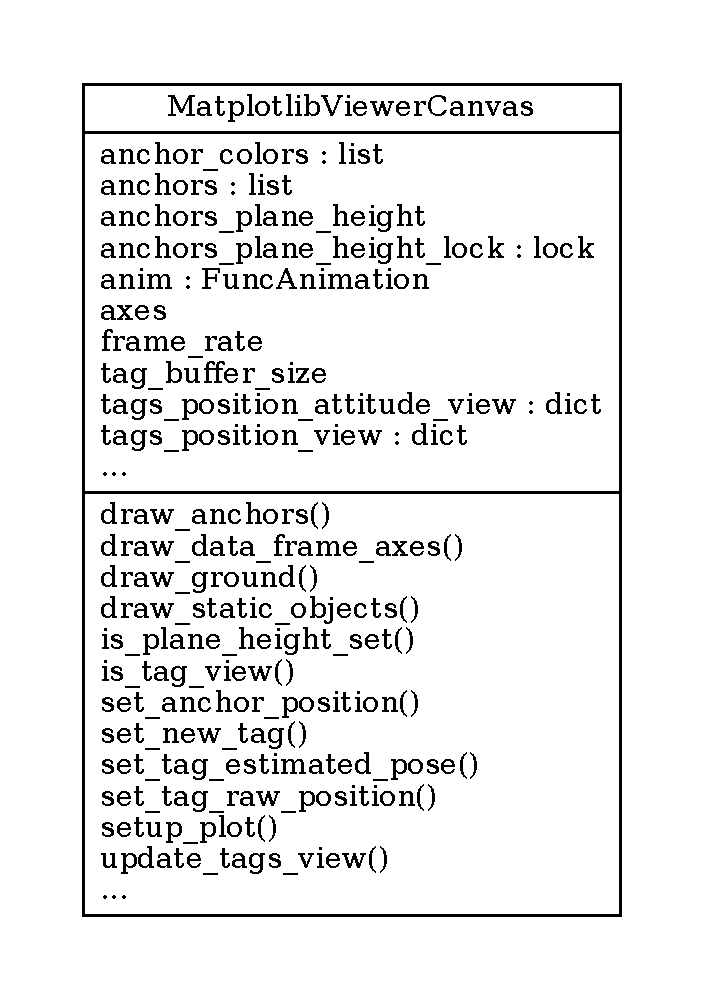
\includegraphics[height=15em]{matplotlib_viewer_canvas}
  \end{center}
  \vskip -3em
  La classe \lstinline!MatplotlibViewerCanvas! si occupa di gestire il Canvas, inserito nella
  finestra principale, che ospita la rappresentazione del tag e delle ancore.\\
  I metodi fondamentali che saranno analizzati sono \lstinline!set_new_tag!, \lstinline!set_tag_raw_position! e  \lstinline!update_tags_view!.
\end{frame}

\begin{frame}[fragile, shrink=15]{Impl.ne - classe \lstinline!MatplotlibViewerCanvas! - \lstinline!set_new_tag!}
  Il metodo \lstinline!set_new_tag! prende come argomenti l'ID del tag \lstinline!tag_ID! ed un colore
  \lstinline!tag_color!.\\
  Queste informazioni sono utilizzate per istanziare due oggetti.\\
  Il TagPositionView utilizzato per conservare in un buffer di grandezza \lstinline!tag_buffer_size! le posizioni risultato
  della trilaterazione eseguita internamente dal tag. Il buffer viene utilizzato per realizzare uno scatter plot 3D con una ``scia''.\\
  Il TagPositionAttitudeView è invece pensato per conservare la stima di posizione e assetto correnti.
  \begin{Python}
    def set_new_tag(self, tag_ID, tag_color):
        self.tags_position_view[tag_ID] = 
             TagPositionView(self.axes,\
                             self.tag_buffer_size,\
                             tag_color)

        self.tags_position_attitude_view[tag_ID] = 
             TagPositionAttitudeView(self.axes,\
                                     tag_color) 
  \end{Python}
\end{frame}

\begin{frame}[fragile, shrink=15]{Impl.ne - classe \lstinline!MatplotlibViewerCanvas! - \lstinline!set_tag_raw_position!}
  Il metodo \lstinline!set_tag_raw_position! prende come argomenti l'ID del tag \lstinline!tag_ID! e le coordinate cartesiane
  \lstinline!x!, \lstinline!y! e \lstinline!z!.

  \begin{Python}
    def set_tag_raw_position(self, tag_ID, x, y, z):
  \end{Python}

  La posizione viene trasformata mediante trasformazione omogenea (\lstinline!vector_hom_transformation!) per tenere conto del fatto
  che i dati sono espressi rispetto ad una terna posizionata all'altezza del piano comune alle
  ancore A0, A1 ed A2. Inoltre, a seconda di come le ancore sono state posizionate, l'asse $z$
  del sistema di riferimento, nel quale sono espresse le posizioni, potrebbe essere rivolto verso il basso.
  In tal caso la parte di rotazione della trasformazione omogenea sarà diversa dalla matrice identità.
  \begin{Python}
        position_data_frame = np.array([[x,y,z]]).T
        position_mpl_frame = self.vector_hom_transformation(position_data_frame)

  \end{Python}
\end{frame}

\begin{frame}[fragile, shrink=10]{Impl.ne - classe \lstinline!MatplotlibViewerCanvas! - \lstinline!set_tag_raw_position!}
  Dopo essere stata trasformata la posizione viene effettivamente memorizzata nel Tag View relativo
  all'ID \lstinline!tag_ID! attraverso la chiamata alla funzione \lstinline!new_position()!
  \begin{Python}
        x = position_mpl_frame.item(0)
        y = position_mpl_frame.item(1)
        z = position_mpl_frame.item(2)
        self.tags_position_view[tag_ID].new_position(x, y, z)
  \end{Python}

  Le funzioni descritte fino a questo punto spiegano, anche se in maniera sintetica,
  il flusso dei dati a partire dalla porta seriale per arrivare alle strutture dati
  che contengono i dati trasformati. Diversi aspetti sono stati trascurati tra cui,
  ad esempio, la gestione vera e propria degli elementi grafici attraverso la libreria
  Matplotlib. Si rimanda al codice per maggiori informazioni.\\
  Per concludere il percorso è necessario descrivere la funzione che si occupa di aggiornare
  periodicamente il Canvas utilizzando i dati disponibili.
\end{frame}

\begin{frame}[fragile, shrink=10]{Impl.ne - classe \lstinline!MatplotlibViewerCanvas! - \lstinline!update_tags_view!}
  La funzione \lstinline!update_tags_view! viene richiamata periodicamente ad una frequenza \lstinline!frame_rate!
  che viene configurata nel metodo \lstinline!setup_plot!
  \begin{Python}
    def setup_plot(self, figure):
        ...
        time_step = 1.0 / self.frame_rate * 1000
        self.anim = animation.FuncAnimation(figure, self.update_tags_view, interval = time_step)
        ...
  \end{Python}

  La funzione \lstinline!update_tags_view! si occupa di richiamare il metodo \lstinline!update_view!
  per ogni TagView e per ogni TagPositionAttitudeView configurato. L'aggiornamento delle View nel tempo
  di fatto realizza l'animazione così come visibile all'utente.
  \begin{Python}
    def update_tags_view(self, frame_number):
        for view_name in self.tags_position_view:
            self.tags_position_view[view_name].update_view()
        for view_name in self.tags_position_attitude_view:
            self.tags_position_attitude_view[view_name].update_view()
  \end{Python}

\end{frame}

